\section{Casimir forces between a conducting plate and a dielectric sphere}
\label{sec:3:casimir-plate-sphere}

An empirical derivation for power law of the casimir energy between a sphere and a conducting plate can be made directly from the energy between two atoms with static polarizability $\alpha_i$ given by Casimir and Polder \cite{Casimir_1948a}. They derived an expression for the Casimir-Polder potential of \footnote{For two macroscopic spheres, the casimir potential looks very similar to eq. \eqref{eq:3:casimir-polder-atom-atom}. The polarizability of a sphere is given by eq. \eqref{eq:3:polarizability-sphere}. Using this result, the Casimir energy between two identical dielectric spheres is given as $-\frac{23\hbar c}{4\pi L^7}\left(\frac{\varepsilon_r-1}{\varepsilon_r+2}\right)^2R^6$. !!!CITATION!!!}
\begin{equation}\label{eq:3:casimir-polder-atom-atom}
  E = -\frac{23\hbar c \alpha_1 \alpha_2}{4 \pi L^7} .
\end{equation}
The polarizability of a sphere with radius $R$ is derived in appendix \ref{apx:polarizability-sphere} and is given for an dielectric with $\varepsilon_r$ as 
\begin{equation} \label{eq:3:polarizability-sphere}
  \alpha_\mathrm{sphere} = \left(\frac{\varepsilon_r-1}{\varepsilon_r+2}\right)R^3 .
\end{equation}
If one atom is now replaced by a conducting sphere ($\varepsilon_r \rightarrow 1$) of radius $\sim L$ (much larger than the atom) with a polarizability of $L^3$, it get obvious that between this big sphere and the atom, the energy is given by a power law of $1/L^4$.
It is therefore natural to assume, that for a macroscopic sphere and a macroscopic plate, the Casimir energy behaves similar to a $1/L^4$ law - at least for the \textit{large separation limit} (LSL).
The exact calculation for this problem is very hard. In fact, no analytic solution is known.

Ford was able to determine an integral expression using a macroscopic approach in 1998 \cite{Ford_1998}:
\begin{multline}
  F = - \frac{\hbar c}{4 \pi L^4} \int_{0}^{\infty} \dd \omega \, \alpha(\omega) \left[3\sin 2 \omega L - 6L\omega \cos 2 \omega L \right. \\ 
  \left. - 6L^2\omega^2 \sin 2 \omega L + 4L^3\omega^3 \cos 2 \omega L\right].
\end{multline}
The expression depends on the polarizability, which is generally not constant for a dielectric. Especially for small separations between the sphere and the plate, this dependence and the non-constant polarizability make this integral nearly unsolvable.
For large separations, much larger than the absorption wavelength of the dielectric or much larger than the wavelength corresponding to the plasma frequency in the Drude-Model, the polarizability can be assumed to be static $\alpha=\mathrm{const}$ \cite{Ford_1998,Kamp_2020}. In this simplifying case, the integral can be solved using an exponential convergence factor and results in
\begin{equation}
  F = -\frac{6 \hbar c}{4 \pi L^5} \alpha
\end{equation}
and thus 
\begin{equation}\label{eq:3:casimir-sphere-plate}
  E = -\frac{3}{8}\frac{\hbar c}{\pi L^4} \left(\frac{\varepsilon_r - 1}{\varepsilon_r + 2}\right)R^3 .
\end{equation}
For the large separation limit, the Casimir interaction between a sphere and a plate behaves like expected considering the motivation of the $1/L^4$-law above in this section.

A second method to calculate the Casimir energy for arbitrary compact objects and a conducting wall was developed by Emig \textit{et. al.} \cite{Emig_2007}. For the sphere-plate geometry, this results in the large separation limit (LSL) in a infinite series, where the first-order term ($\propto 1/L^4$) is precisely given by eq. \eqref{eq:3:casimir-sphere-plate}. The first 8 terms of this series are shown in \cref{fig:3:casimir-behavior} as well as a few specific numerical points for higher terms.
\begin{figure}[!ht]
  \centering
  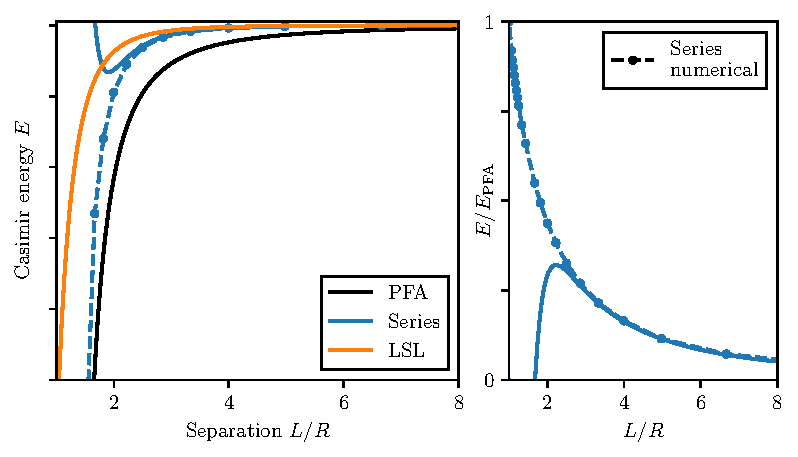
\includegraphics[width=\textwidth]{./../figures/casimir-behavior.pdf}
  \caption{Behavior of different approximations of the casimir interaction between a conducting sphere and a perfectly conducting plate. Additionally, a comparison between the PFA and an exact numerical series expansion from Ref. \cite{Emig_2007a} is shown.}
  \label{fig:3:casimir-behavior}
\end{figure}
It becomes evident, that the series expansion converges to the LSL eq. \eqref{eq:3:casimir-sphere-plate} for large separations and to the PFA eq. \eqref{eq:3:PFA-sphere-plate} for small separations.
However, quantitatively the numerics show, that $E/E_\mathrm{PFA} \leq 1$ and thus the PFA predicts a stronger Casimir energy fir all separations.
\begin{theorem}
  The PFA model for a \emph{conducting sphere} and a conducting plate predicts a stronger casimir energy for all separations $L/R$ than the LSL or the exact series expansion.
\end{theorem}
\begin{proof}
  a) The numerical series expansion in \cref{fig:3:casimir-behavior} from Ref. \cite{Emig_2007a} shows that $\abs{E_\mathrm{series}} \leq \abs{E_\mathrm{PFA}}$ for all $L/R$.

  b) Comparing the PFA eq. \eqref{eq:3:PFA-sphere-plate} for a conducting sphere with a dielectric one, it becomes evident, that $\abs{E_\mathrm{cond.}} \geq \abs{E_\mathrm{diel.}}$. This can be seen by the fact that for $\varepsilon_r \in [1, \infty)$ $\varphi(\varepsilon_r) \leq 1$ and $(\varepsilon_r - 1)/(\varepsilon_r - 1) \leq 1$. Thus the PFA for conductors is always a worse approximation. 

  c) Analytically, it can be shown that the energy predicted by the LSL eq. \eqref{eq:3:casimir-sphere-plate} is always smaller than the PFA:
  \begin{align}
    \abs{E_\mathrm{PFA}} &> \abs{E_\mathrm{LSL}}\\
     \frac{\hbar c \pi^3}{720} \left(\frac{\varepsilon_r - 1}{\varepsilon_r + 1}\right)\varphi(\varepsilon_r) \frac{R}{\mathscr{L}^2} &> \frac{3\hbar c}{8 \pi L^4}\left(\frac{\varepsilon_r - 1}{\varepsilon_r + 2}\right) R^3 \\
    \frac{8 \pi^4}{3 \cdot 720} \frac{\varepsilon_r + 2}{\varepsilon_r + 1} \varphi(\varepsilon_r) &> \frac{(L-R)^2 R^2}{L^4} = \left(\frac{R}{L}\right)^2 - 2\left(\frac{R}{L}\right)^3 + \left(\frac{R}{L}\right)^4
  \end{align}
  Maximizing the RHS, and using the fact that $R/L \leq 1$, the maximum is $1/16$ at $R/L=1/2$. The minimum of the LHS is a little more complicated. The minimum of $\varphi(\varepsilon_r)$ is reached for $\varepsilon_r = 1$ and is at a minimum $0.46$. The minimum of $(\varepsilon_r + 2)/(\varepsilon_r + 1)$ is reached at $\varepsilon_r \rightarrow \infty$ and is $1$. Thus the LHS is at the absolute (unreachable) minimum $8\pi^4/2160 \cdot 0.46 \approx 0.166$ which is still larger than $1/16$.
\end{proof}
\begin{remark}
  This is rather unintuitive, because one would expect it to be the other way around. The $1/L^4$ dependence in the LSL should - for small separations - tend much faster to zero than the $1/\mathscr{L}^2$ dependence in the PFA. However considering the differences between $L$ and $\mathscr{L} = L-R$, this is no longer surprising.
\end{remark}
Admittedly, for separations $L/R \gtrsim 2$, the difference is not very large. Nevertheless will I use the PFA eq. \eqref{eq:3:PFA-sphere-plate} for the rest of the thesis as a worst-case estimation. Keep in mind, that the some quantities might be overestimated.
